\section*{Problems}
\addcontentsline{toc}{section}{Problems}

\begin{problem}
	In class, we have seen how to formulate a second-quantized version of the Hamiltonian of a non-relativistic many-particle system in a general basis,
	\begin{eqnarray}
		H = \sum_{\lambda_1,\lambda_2} ~ \varepsilon_{\lambda1,\lambda_2}~ c^{\dagger}_{\lambda_1}  c_{\lambda_2} 
		+ \sum_{\lambda_1,\lambda_2\lambda_3,\lambda_4}
		~v_{\lambda_1,\lambda_2\lambda_3,\lambda_4}~
		c^{\dagger}_{\lambda_1} ~ c^{\dagger}_{\lambda_2}  c_{\lambda_3} ~ c_{\lambda_4}  \nonumber
	\end{eqnarray}
	where $\varepsilon_{\lambda_1,\lambda_2}$ and $v_{\lambda_1,\lambda_2\lambda_3,\lambda_4}$ are matrix elements of the one-particle and two-particle contributions to the Hamiltonian, computed using a complete set of basis functions $\{ \phi_{\lambda}(x) \}$.
	\ \\
	\ \\
	{\bf a)} Write down an expression for the Hamitonian in a general basis for the case where the system is materially open and coupled to particle reservoir. (In the above version, it is materially closed).
	\ \\
	\ \\
	{\bf b) } Give an explicit form of this   Hamiltonian using a Bloch-basis for $\{ \phi_{\lambda}(x) \}$
	\begin{eqnarray}
		\phi_{\lambda}(x) = \phi_{{\bf k},\sigma}({\bf r},s)  = \frac{1}{\sqrt{V}} ~e^{i {\bf k} \cdot {\bf r}} ~ u_{\bf k} ({\bf r}) ~ \chi_{\sigma}(s) \nonumber
	\end{eqnarray}
	in the notation used in class. (Hint: The Bloch functions may be taken to be eigenfunctions of the one-particle problem). 
\end{problem}
\begin{problem}
	
	Show by an explicit calculation that the following relations hold for the spin-part of the wavefunction $\chi_\sigma(s)$ of $S=1/2$ particles:
	\begin{eqnarray}
		\sum_{\sigma} \chi^*_\sigma(s)  \chi_\sigma(s^{\prime}) & = & \delta_{s,s^{\prime}} \nonumber \\
		\sum_{s} \chi^*_\sigma(s)  \chi_{\sigma^{\prime}}(s) & = & \delta_{\sigma,\sigma^{\prime}} \nonumber
	\end{eqnarray}
\end{problem}
\begin{problem}
	
	Consider the following two-body potential that could enter into the two-particle contribution to a many-body Hamiltonian
	\begin{eqnarray}
		V({\bf r}) = V(r) = \frac{A}{r} ~ \exp(-r/\lambda_{TF}) \nonumber 
	\end{eqnarray} 
	Compute the Fourier-transform of this potential. Give an interpretation of the quantity $\lambda_{TF}$. Here $A$ is a dimensionful constant that we need not specify further. 
\end{problem}

% HWP 2

\begin{problem}
	
	Consider a tight binding Hamiltonian with nearest-neighbor hopping on a general two dimensional Bravais lattice with $N$ lattice points, in contact with a particle reservoir. The chemical potential of the system is denoted $\mu$. The nearest-neighbor hopping element is given by $t$. The Hamiltonian is given by 
	\begin{eqnarray}
		H = - t \sum_{\langle i,j \rangle, \sigma} c^{\dagger}_{i,\sigma} c_{j,\sigma} - \mu   \sum_{ i, \sigma} c^{\dagger}_{i,\sigma} c_{i,\sigma} \nonumber 
	\end{eqnarray}
	Here, $(c^{\dagger}_{i,\sigma}, c_{i,\sigma})$ create and destroy particles in spin-state $\sigma$ on site $i$. 
	Introduce Fourier-transformed operators 
	\begin{eqnarray}
		c^{\dagger}_{{\bf k},\sigma} & = & \frac{1}{\sqrt{N}} \sum_{i} c^{\dagger}_{i,\sigma} ~ \e^{-i {\bf k} \cdot {\bf r}_i} \nonumber  \\
		c_{{\bf k},\sigma} & = & \frac{1}{\sqrt{N}} \sum_{i} c_{i,\sigma} ~ \e^{i {\bf k} \cdot {\bf r}_i} \nonumber
	\end{eqnarray}
	where ${\bf r}_i$ is the position at lattice site $i$. 
	\ \\
	\ \\
	{\bf a)} Show that Hamiltonian may be written on form
	\begin{eqnarray}
		H = \sum_{{\bf k}, \sigma} E_{\bf k} ~ c^{\dagger}_{{\bf k},\sigma} c_{{\bf k},\sigma}  \nonumber 
	\end{eqnarray}
	and give an expression for $E_{\bf k}$ for a general two-dimensional Bravais lattice. 
	\ \\
	\ \\
	{\bf b)} Specialize to the case of a two-dimensional square lattice, see Figure \ref{fig:squareblattice}, and give the expression for $E_{\bf k}$ in this case.
	\missingfig{Missing fig: Square lattice}
	%\begin{figure}[htb]
	%	\centering
	%	\includegraphics[width = 0.35\textwidth]{main_1.pdf}
	%	\caption{Square lattice.}
	%	\label{fig:squareblattice}
	%\end{figure}
	
	\newpage
	\ \\
	\ \\
	{\bf c)} Imagine that we now consider a model on a {\it honeycomb} lattice, see Figure \ref{fig:honeycomblattice}.   Explain what the {\it principal} difference between this lattice and the square lattice is.
	\missingfig{Missing fig: Honeycomb lattice}
	%\begin{figure}[htb]
	%	\centering
	%	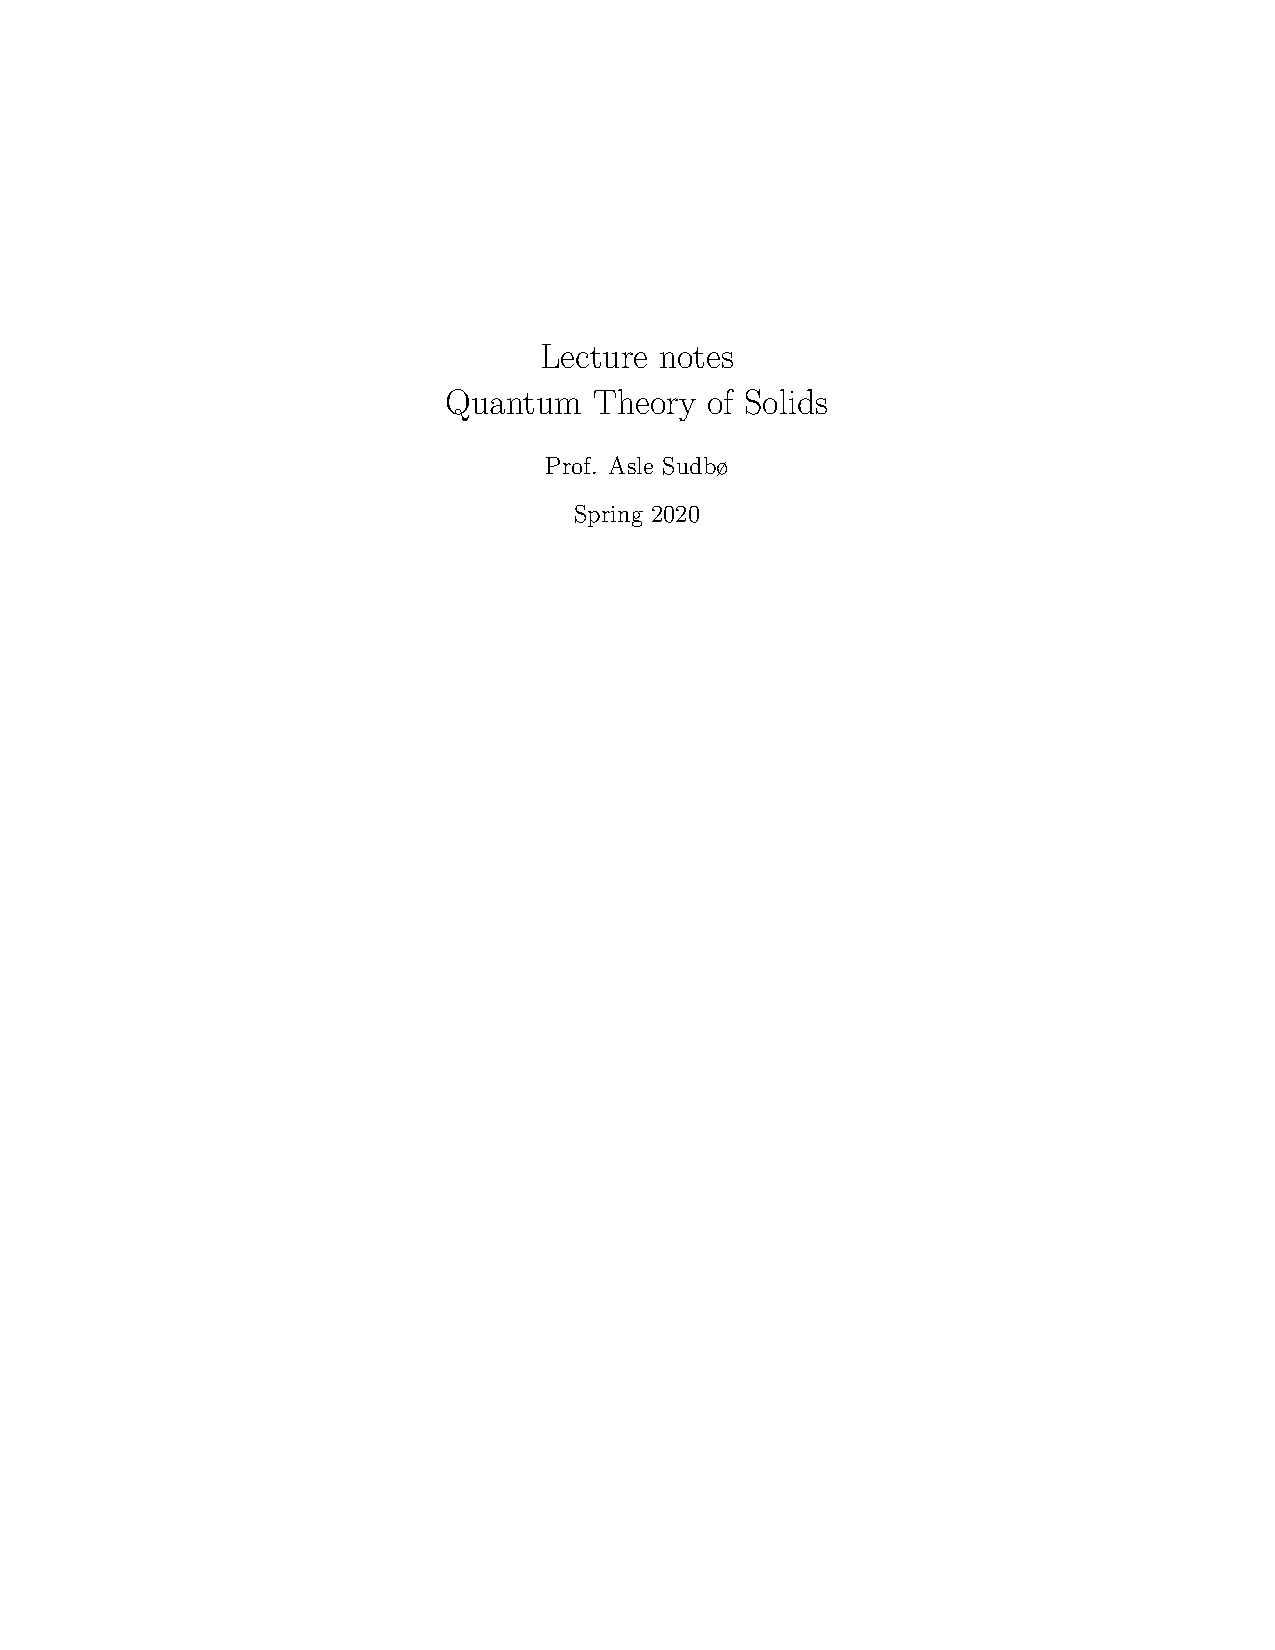
\includegraphics[width = 0.45\textwidth]{main.pdf}
	%	\caption{Honeycomb lattice.}
	%	\label{fig:honeycomblattice}
	%\end{figure}
	\ \\
	\ \\
	{\bf d)}  Write down a tight-binding model for this system, conidering only nearets neighbor interactions, and find $E_{\bf k}$. (Hint: You need to introduce two distinct types of fermions, one type for the red atoms and one type for the blue atoms). 
\end{problem}

\begin{problem}
	Consider a tight-binding model in a uniform external magnetic field $h$ directed along the z-direction.
	The Hamiltonian is given by 
	\begin{eqnarray}
		H = - t \sum_{\langle i,j \rangle, \sigma} c^{\dagger}_{i,\sigma} c_{j,\sigma} - \mu   \sum_{ i, \sigma} c^{\dagger}_{i,\sigma} c_{i,\sigma}
		- h \sum_{i, \sigma} \sigma c^{\dagger}_{i \sigma}  c_{i \sigma}  
		\nonumber 
	\end{eqnarray}
	in the same notation as in Problem 1. The last term is the second-quantized version of the Zeeman-term 
	$- {\bf h} \cdot {\bf S} = - h \sum_i S_{i z} = - h \sum_{i} \left[ c^{\dagger}_{i,\uparrow} c_{j,\uparrow}- c^{\dagger}_{i,\downarrow} c_{j,\downarrow} \right] =-  h \sum_{i, \sigma} \sigma c^{\dagger}_{i \sigma}  c_{i \sigma}.$
	\ \\
	\ \\
	{\bf a)} Introduce the same Fourier-transform as in Problem 1, and show that the Hamiltonian may be written on the form
	\begin{eqnarray}
		H = \sum_{{\bf k},\sigma} ~ E_{\bf k, \sigma} ~ c^{\dagger}_{{\bf k},\sigma} c_{{\bf k},\sigma}  \nonumber 
	\end{eqnarray}
	and give an expression for $E_{{\bf k},\sigma}$ for a general two-dimensional Bravais lattice. 
	\ \\
	\ \\
	{\bf b)}  Consider instead  another variant of the tight-binding model, now in the absence of a magnetic field, but with a spin-dependent hopping matrix element. (In lectures Week 4, we discuss what the origin of such spin-dependent hopping could be). The Hamiltonian is given by, with a general spin-dependent hopping matrix element $ t^{\sigma \sigma^{\prime}}_{ij}$
	\begin{eqnarray}
		H = -  \sum_{\langle i,j \rangle, \sigma, \sigma^{\prime}} t^{\sigma \sigma^{\prime}}_{ij}c^{\dagger}_{i,\sigma^{\prime}} c_{j,\sigma} - \mu   \sum_{ i, \sigma} c^{\dagger}_{i,\sigma} c_{i,\sigma}
		\nonumber 
	\end{eqnarray}
	Consider a special case $ t^{\sigma \sigma^{\prime}}_{ij} = t^{\sigma \sigma}_{ij} \delta_{\sigma,\sigma^{\prime}}$, with 
	$t_{ij}^{\uparrow \uparrow} \neq t_{ij}^{\downarrow \downarrow}$.  Introduce the same Fourier-transform as in Problem 1, and show that the Hamiltonian may be written on the form
	\begin{eqnarray}
		H = \sum_{{\bf k},\sigma} ~ E_{\bf k, \sigma} ~ c^{\dagger}_{{\bf k},\sigma} c_{{\bf k},\sigma}  \nonumber 
	\end{eqnarray}
	and give an expression for $E_{{\bf k},\sigma}$ for a general two-dimensional Bravais lattice. 
	\ \\
	\ \\
	{\bf c)} Compare with the results in Problem 2 {\bf a)}, and show that this sort of spin-dependent hopping may be interpreted as particles moving in  a {\bf k}-dependent external magnetic field along the $z$-axis.  
\end{problem}

% HWP 3
\begin{problem}
	
	A non-interacting electron gas has a Hamiltonian which in a grand canonical ensemble may be written on the form
	\begin{eqnarray}
		H = \sum_{{\bf k},\sigma} ~ \left( \varepsilon_{{\bf k}} - \mu \right) ~ c^{\dagger}_{{\bf k}, \sigma}    c_{{\bf k}, \sigma}   \nonumber
	\end{eqnarray}
	where $\varepsilon_{{\bf k}}$ is the single-particle excitation energy and $\mu$ is a chemical potential. Let us now subject this system to magnetic field directed along, say, the $\hat z$-axis. This adds a term $- {\bf B}\cdot {\bf S}$ to the Hamiltonian. Here, ${\bf S}$ is the total spin of the system, ${\bf S} = \sum_i {\bf S}_i$ for spins ${\bf S}_i$ on lattice site $i$. 
	We have seen in HW $\#$ 2 that  $H$ may be written on the form
	\begin{eqnarray}
		H = \sum_{{\bf k},\sigma} ~ \left( \varepsilon_{{\bf k}} - \mu_\sigma \right) ~ c^{\dagger}_{{\bf k}, \sigma}    c_{{\bf k}, \sigma}   \nonumber
	\end{eqnarray}
	where $\mu_\sigma = \mu + \sigma B$.
	\ \\
	\ \\
	{\bf a)} Denote the spin-dependent density of states of this system by $D_\sigma(\omega)$, where
	\begin{eqnarray}
		D_\sigma(\omega) = \frac{1}{N} ~ \sum_{{\bf k}} ~\delta(\omega -( \varepsilon_{{\bf k}} - \mu_\sigma  )) \nonumber
	\end{eqnarray} 
	Let $\varepsilon_{{\bf k}} = \hbar^2 k^2/2m$. Compute $D_\sigma(\omega)$ in $2$ and $3$ dimensions. (Hint: Convert the summation over ${\bf k}$ to a $d$-dimensional integral 
	$$ \sum_{{\bf k}} \to (L/a)^d \int d^d k/(2\pi)^d$$ 
	Here $N$ is the number of lattice sites, $a$ is the lattice constant of the lattice, and $L$ is the sidelength of the volume $V$ of the system, $V=L^d$. )  
	\ \\
	\ \\
	{\bf b)} Compute the zero-temperature magnetization of this system, $M = N_{\uparrow}- N_{\downarrow}$, where $N_\sigma$ is the total number of particles with spin $\sigma$ in the system. (Hint: Here you must invoke the Pauli principle and occupy states up to some maximum energy, say $\varepsilon_F$, which will determine the total number of particles $N=N_{\uparrow}+ N_{\downarrow}$ in the system. Express therefore your answer also in terms of $\varepsilon_F$.)
\end{problem}
\begin{problem}
	
	
	Consider a $S=1/2$ fermionic  tight-binding model on a two-dimensional square lattice with $N$ lattice sites, describing a spin-orbit coupled system in an external magnetic field, given by the Hamiltonian 
	\begin{align}
		\begin{split}
			H =&   \sum_{\langle ij \rangle} 
			\begin{pmatrix} c_{i\uparrow}^\dagger & c_{i\downarrow}^\dagger  \end{pmatrix}
			\begin{pmatrix} -t & s_{ij}^{\uparrow\downarrow} \\ s_{ij}^{\downarrow\uparrow} & -t \end{pmatrix}  
			\begin{pmatrix} c_{j\uparrow} \\ c_{j\downarrow}  \end{pmatrix}
			- \sum_{i \sigma} \mu_\sigma n_{i\sigma} \nonumber 
		\end{split}
	\end{align}
	Here,  $\langle i,j \rangle$ denotes that $i$ and $j$ are nearest neighbor lattice sites on the square lattice. $\mu_{\sigma}$ is the chemical potential for particles with spin $\sigma$, $c^{+}_{i,\sigma}, c_{i,\sigma}$ are fermionic creation and destruction 
	operators, and $n_i = \sum_{\sigma} n_{i \sigma}$ are number operators, $n_{i \sigma} = c^{+}_{i,\sigma} c_{i,\sigma}$. $t$ represents a nearest-neighbor hopping without spin-flip in the hopping process, 
	while $ s_{ij}^{\uparrow\downarrow} = (s_{ji}^{\downarrow\uparrow} )^*$ represents a nearest-neighbor spin-flipping hopping elements (spin-orbit coupling) which depend on the direction of the vector that connects lattice site $i$ with lattice site $i$, 
	$s_{ij}^{\downarrow\uparrow} =s_{i, i+\delta}^{\downarrow\uparrow} = s_{\delta} $ where $\delta$ is a unit vector in $x$- or $y$-direction.  For Rashba spin-orbit coupling (see lecture notes Week 4), we set $s_{\pm \hat{ x}} = \mp i \eta$ 
	and $s_{\pm \hat{y}}= \pm \eta$. 
	\ \\
	\ \\
	{\bf a)} Introduce Fourier-transformed fermion operators 
	\begin{eqnarray}
		c^{+}_{{\bf k},\sigma} & = & \frac{1}{\sqrt{N}} \sum_i c^{+}_{i,\sigma} e^{-i {\bf k} \cdot {\bf r}_i} \nonumber \\
		c_{{\bf k},\sigma} & = & \frac{1}{\sqrt{N}} \sum_i c_{i,\sigma} e^{i {\bf k} \cdot {\bf r}_i} \nonumber
	\end{eqnarray}
	where ${\bf r}_i$ is the position on the lattice corresponding to lattice site $i$. Show that the Hamitonian given above may be written on the form
	\begin{align}
		\begin{split}
			H =&   \sum_{{\bf k}} 
			\begin{pmatrix} c_{k\uparrow}^\dagger & c_{k \downarrow}^\dagger  \end{pmatrix}
			\begin{pmatrix} \varepsilon_{{\bf k}}-\mu - h & \gamma_{{\bf k}} \\ \gamma_{{\bf k}}^{*} & \varepsilon_{{\bf k}} - \mu + h \end{pmatrix}  
			\begin{pmatrix} c_{k \uparrow} \\ c_{ k\downarrow}  \end{pmatrix}
		\end{split} \nonumber 
	\end{align}
	and give expressions for $\varepsilon_{{\bf k}}, \gamma_{{\bf k}}, \gamma_{{\bf k}}^{*}$ as well as $\mu$ and $h$, in terms of the parameters of the Hamiltonian.  
	\ \\
	\ \\
	{\bf b)} This Hamiltonian may further be diagonalized in terms of new fermion operators $\alpha^{\pm}_{{\bf k}}$ and $\alpha^{\dagger \pm}_{{\bf k}}$. Show, by introducing the unitary transformation
	\begin{eqnarray}
		S = \frac{1}{\sqrt{r_{{\bf k}}^2  + | \gamma_{{\bf k}} |^2}}\begin{pmatrix} r_{{\bf k}} & \gamma_{{\bf k}} \\ \gamma_{{\bf k}}^{*} & -r_{{\bf k}} \end{pmatrix}  \nonumber 
	\end{eqnarray}
	that the Hamiltonian may be written on the form
	\begin{eqnarray}
		H & =&   \sum_{{\bf k}} 
		\begin{pmatrix} c_{k\uparrow}^\dagger & c_{k \downarrow}^\dagger  \end{pmatrix} S S^{-1}
		\begin{pmatrix} \varepsilon_{{\bf k}}-\mu - h & \gamma_{{\bf k}} \\ \gamma_{{\bf k}}^{*} & \varepsilon_{{\bf k}} - \mu + h \end{pmatrix}   S S^{-1}
		\begin{pmatrix} c_{k \uparrow} \\ c_{ k\downarrow}  \end{pmatrix} \nonumber \\
		& = &  \sum_{{\bf k}}  \left[  E^{+}_{{\bf k}} ~ \alpha^{\dagger +}_{{\bf k}} \alpha^{+}_{{\bf k}} 
		+ E^{-}_{{\bf k}} ~ \alpha^{\dagger -}_{{\bf k}} \alpha^{-}_{{\bf k}} \right]  \nonumber
	\end{eqnarray}
	and give expressions for $ E^{\pm}_{{\bf k}}$. Here, $r_{{\bf k}} =- h + \sqrt{h^2+|\gamma_{{\bf k}}|^2}$. 
	\ \\
	\ \\
	{\bf c)} The spectrum of these particles in general have global minima at four distinct finite ${\bf k}$, provided that the Zeeman-field is not too large. Give 
	a physical interpretation of the fact that the lowest energy state is located at these finite wave-vectors 
	(momenta). (Hint: Think about what a state with a finite momentum represents). 
\end{problem}




